
\documentclass[main.tex]{subfiles}
\begin{document}
	
	\chapter{NLP}
	\chapterauthor{Paul Schnipper}
    \section{Using Julius on the HSR}
        The groups main goal for the NLP was to actually become part of the main demonstration and to run during the RoboCup. For this the group investigated method of loading dictionaries onto the HSR. But dew to the Corona-Virus were never actually able to perform any speech recognition on the robot directly.
    \section{Implementing basic commands}
        To allow the planning group to test the integration of hard commands into the highlevel plans. Multiple options for running the speech-recognition while running the simulation. While in practice most often only bagfiles containing the output from Julius was used. This way at least the textparser, actually ran. Although it was also possible and tested in that way, that Julius was run locally and connected to the Simulator through the VPN Tunnel. but dew to Julius being inaccurate with different microphones then the HSRs, this method wasn't used on a regular basis.
    \section{The QA-System Demo}
        \begin{figure}[H]
            \centering
            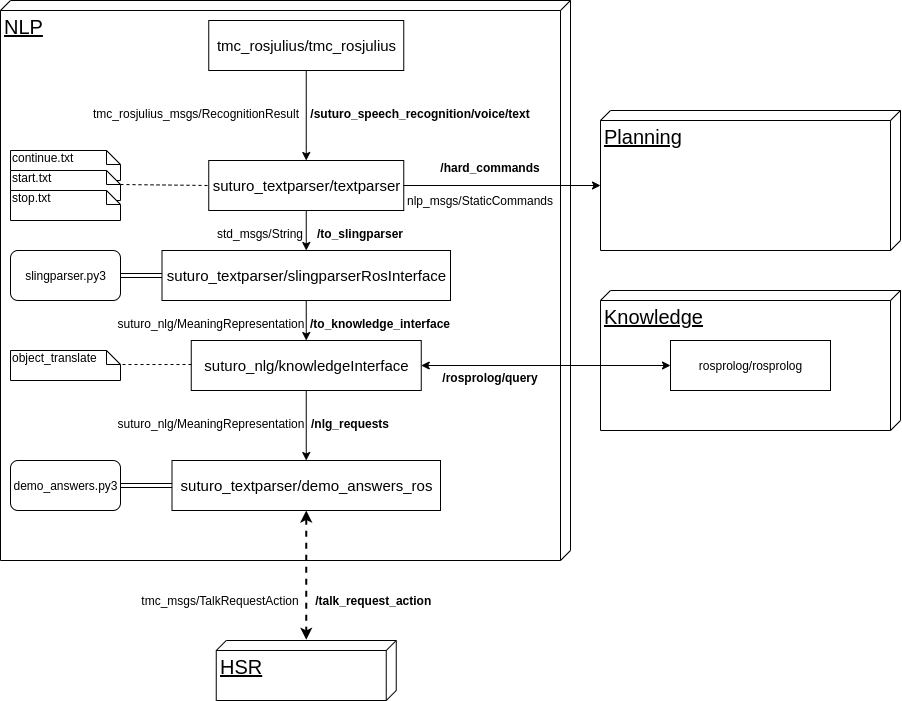
\includegraphics[width=1.2\linewidth]{architecture/nlp}
            \caption{}
            \label{fig:nlp}
        \end{figure}
        \subsection{knowledge interface}
            The knowledge interface node has been created to enable the QA-system demo. Its code is explained in the final documentation. It works through basic rosprolog queries. Because the spoken word for objects are different to the ID's used by the knowledge system a bidirectional translation had been added. This uses a csv style file with the spoken representation in one column and the ID in a different column. For example:
            \begin{verbatim}
instant coffee powder,Magicokaffetypfamilycappuccino
red pringles can,Pringlesoriginal
cup,Cup

            \end{verbatim}
        \subsection{demo answers generator}
            The \texttt{demo answer generator} takes the \texttt{MeaningRepresentation} message produced by the Knowledge interface and creates a speakable sentence out off it. Originally the idea was for the speech generation to be done using the simplenlg python library, witch is only usable in Python3. To prepare for this, the \texttt{demo\_answers\_ros} and \texttt{demo\_answers.py3} were created. But dew to time constrains \texttt{demo\_answers.py3} was actually only filled with simple text generation based on String concatenation. SimpleNLG would have enabled correct articles to be used.
    
    	
\end{document}
